\section{Технологический раздел}

\subsection{Выбор и обоснование языка и среды программирования}
При написании программного кода использовался язык программирования C \cite{cLanguage}.

В качестве среды разработки использовалась ``Visual Studio Code'' \cite{VSCode}.

Данный выбор обусловлен следующими факторами:
\begin{itemize}
\item наличие плагинов для написания программ, работающих на уровне ядра,
\item широкий функционал,
\item программное обеспечение с открытым исходным кодом.
\end{itemize}

\subsection{Реализация алгоритмов определения и логирования приоритетов, времени выполнения и простоя процессов.}
В листинге \ref{code:loggingModule} предоставлена реализация алгоритмов определения и логирования приоритетов, времени выполнения и простоя процессов.
\begin{code}
	\captionof{listing}{Реализация алгоритмов определения и логирования приоритетов, времени выполнения и простоя процессов.}
	\label{code:loggingModule}
	\inputminted
	[
	frame=single,
	framerule=0.5pt,
	framesep=20pt,
	fontsize=\small,
	tabsize=4,
	linenos,
	numbersep=5pt,
	xleftmargin=10pt,
	firstline=43,
	lastline=113,
	breaklines=true
	]
	{text}
	{code/oldMd.c}
\end{code}

\subsection{Реализация алгоритма предоставления информации о процессах пользователю}
В листинге \ref{code:starterLogger} предоставлена реализация алгоритма предоставления информации о приоритетах, времени выполнения и простоя процессов пользователю.

\begin{code}
	\captionof{listing}{Реализация алгоритма предоставления информации о приоритетах, времени выполнения и простоя процессов пользователю.}
	\label{code:starterLogger}
	\inputminted
	[
	frame=single,
	framerule=0.5pt,
	framesep=20pt,
	fontsize=\small,
	tabsize=4,
	linenos,
	numbersep=5pt,
	xleftmargin=10pt,
	firstline=17,
	lastline=48,
	breaklines=true
	]
	{text}
	{../../src/starterLogger.c}
\end{code}

\subsection{Makefile}
В листинге \ref{code:Makefile} предоставлено содержание Makefile для сборки компонентов.

\begin{code}
	\captionof{listing}{Содержание Makefile.}
	\label{code:Makefile}
	\inputminted
	[
	frame=single,
	framerule=0.5pt,
	framesep=20pt,
	fontsize=\small,
	tabsize=4,
	linenos,
	numbersep=5pt,
	xleftmargin=10pt,
	%firstline=24,
	%lastline=25,
	breaklines=true
	]
	{text}
	{../../src/Makefile}
\end{code}

\subsection{Демонстрация работы}
На рисунках \ref{fig:firstIt}--\ref{fig:thirdIt} предоставлена демонстрация работы программы загрузки модуля и получения информации.

На рисунке \ref{fig:dmesg} предоставлено содержание журнала ядра при загрузке и выгрузке модуля из системы.

\begin{figure}[H]
	\centering
	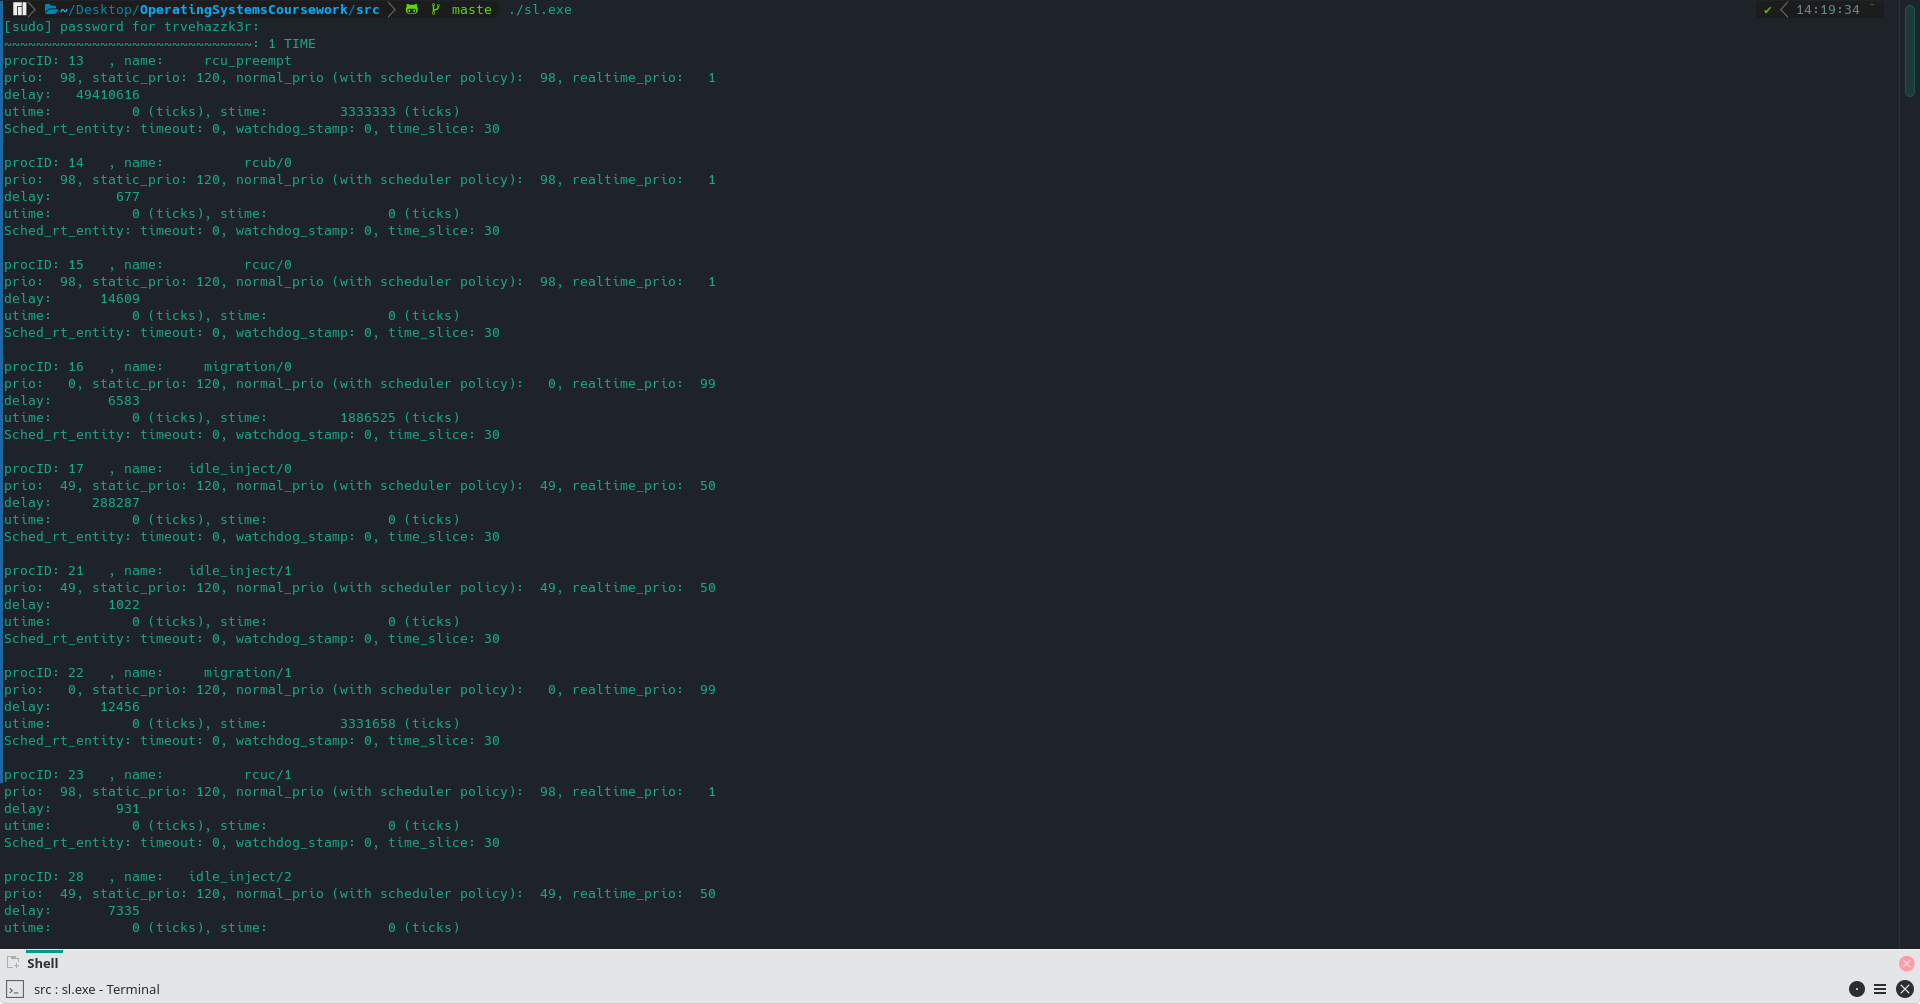
\includegraphics[scale=0.8]{img/firstIt.png}
	\caption{Вывод при запуске starterLogger.c (первая итерация). }
	\label{fig:firstIt}
\end{figure}

\begin{figure}[H]
	\centering
	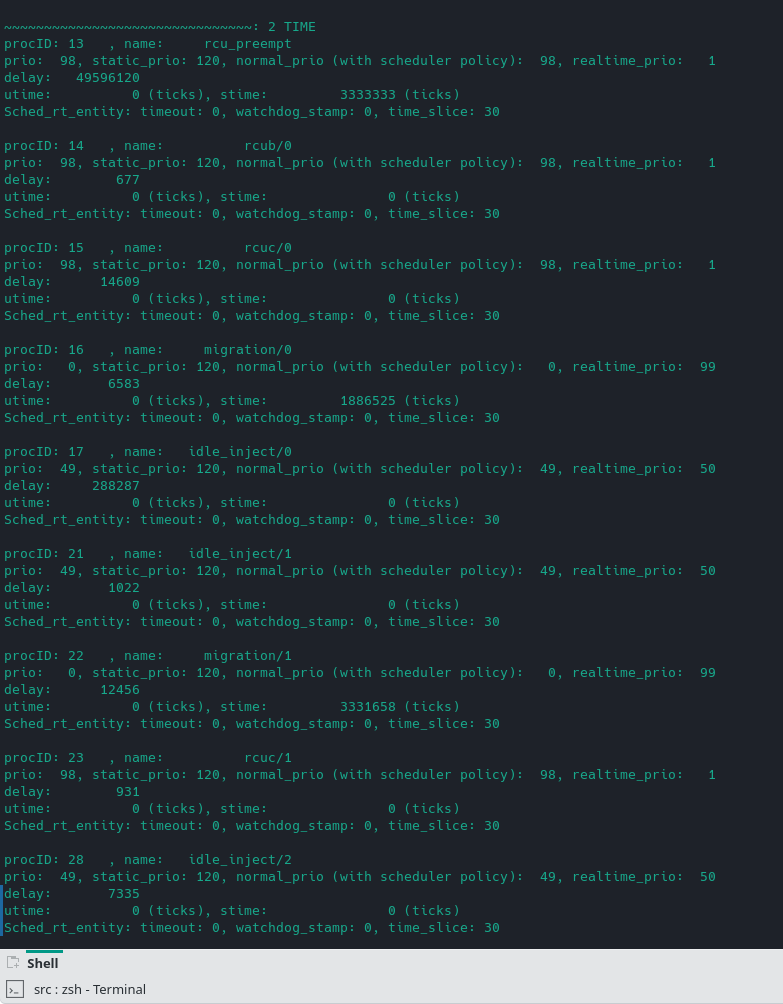
\includegraphics[scale=0.8]{img/secondIt.png}
	\caption{Вывод при запуске starterLogger.c (вторая итерация). }
	\label{fig:secondIt}
\end{figure}

\begin{figure}[H]
	\centering
	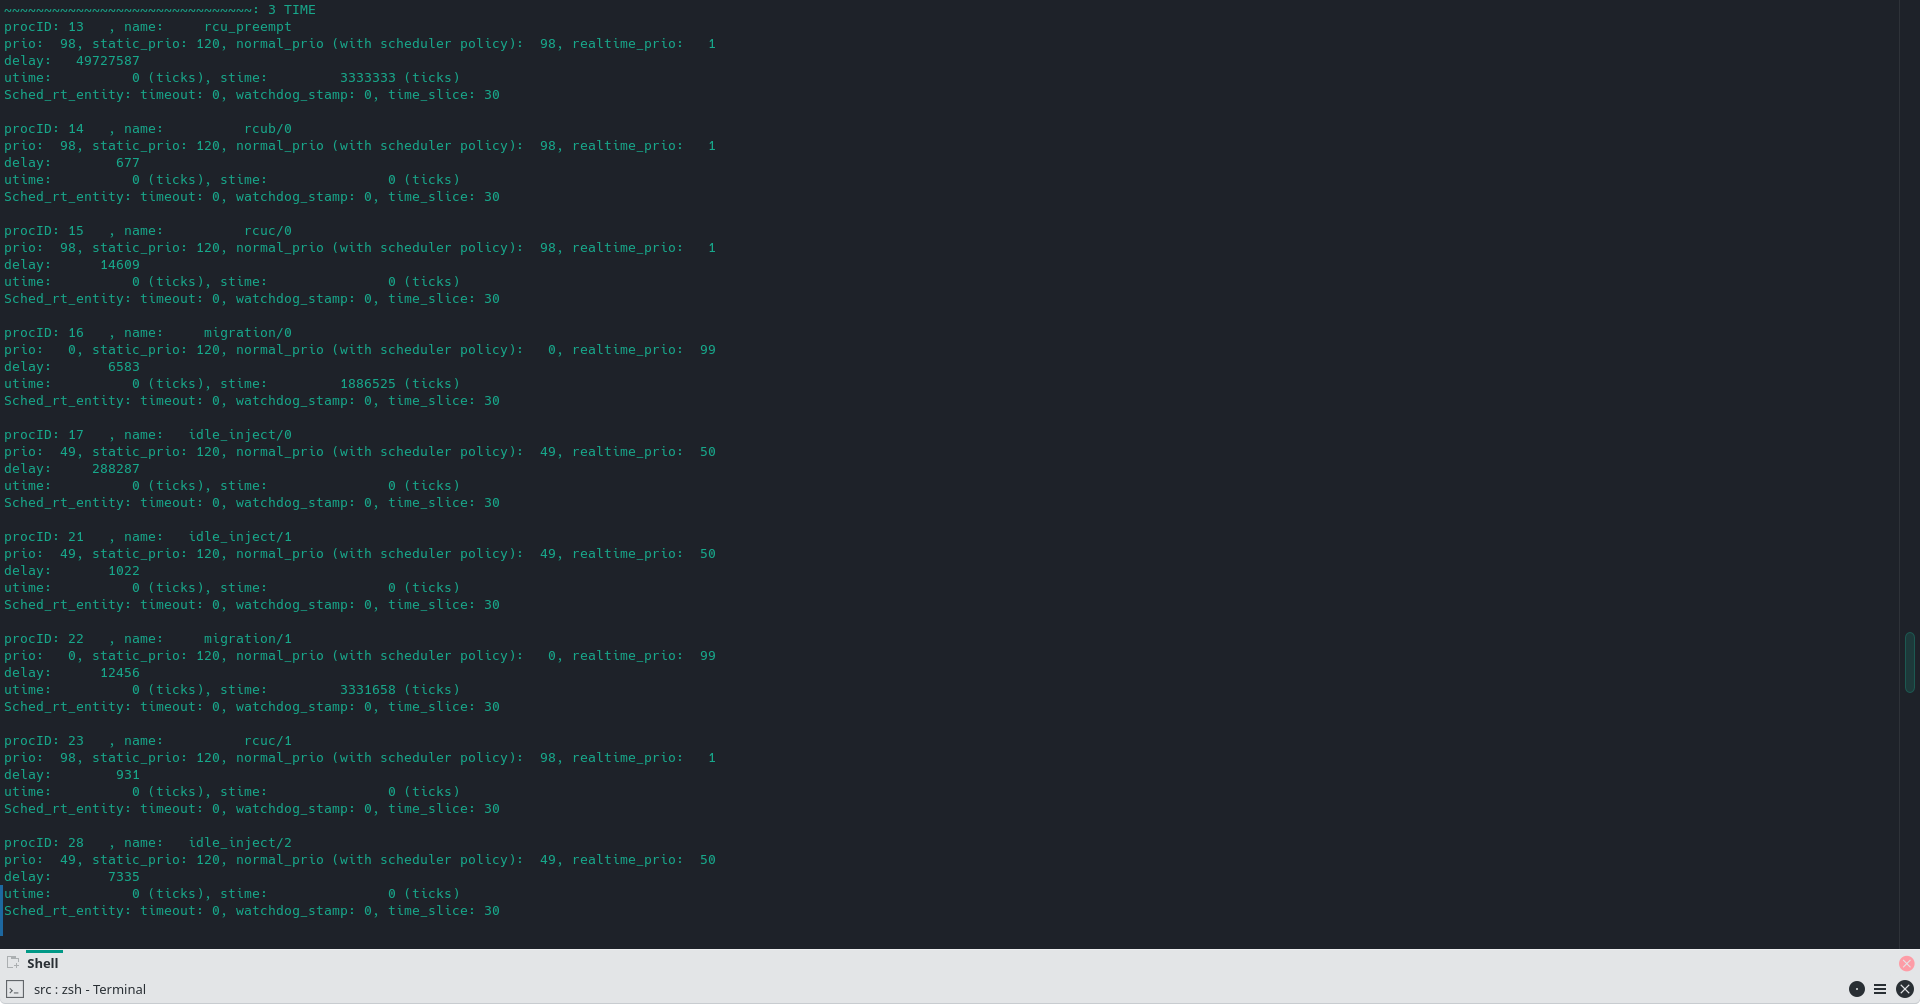
\includegraphics[scale=0.8]{img/thirdIt.png}
	\caption{Вывод при запуске starterLogger.c (третья итерация). }
	\label{fig:thirdIt}
\end{figure}

\begin{figure}[H]
	\centering
	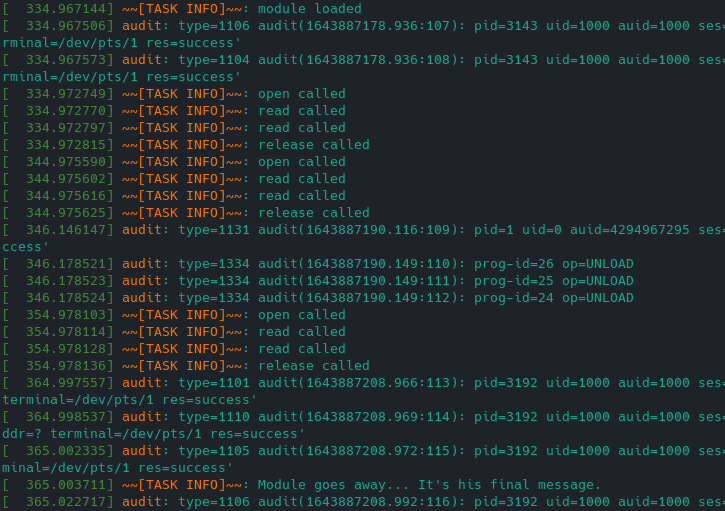
\includegraphics[scale=0.8]{img/dmesg.png}
	\caption{Содержание журнала ядра. }
	\label{fig:dmesg}
\end{figure}